%-----------------------------------------------
% Dateiname: Doctrine.tex
% Autor    : Stefano Kowalke <blueduck@gmx.net>
% Lizenz   : BSD
%-----------------------------------------------
\section{Doctrine}
\label{basics:sec:doctrine}
Das Doctrine Projekt besteht aus einer Reihe von PHP-Bibliotheken, die Schnittstellen rund um die Datenbankschicht bereitstellen. Die Konzepte sind beeinflusst von Javas \textit{Hibernate}\footnote{\url{http://hibernate.org/}} (vgl. \cite{web:t3nDoctrine2009}).

Das Projekt wurde 2006 von Konsta Vesterinen initiiert\footnote{\url{http://docs.doctrine-project.org/projects/doctrine1/en/latest/en/manual/acknowledgements.html}} und im Jahr 2008 als Version 1.0.0 veröffentlicht.

Die beiden bekanntesten Produkte des Projekts sind:
\begin{itemize}
	\item \gls{orm} - ermöglicht die objektrelationale Abbildung von Objekten auf Datenbanktabellen
	\item \gls{dbal} - stellt eine Datenbankabstraktionsschicht bereit
\end{itemize}

Wie aus Abbildung~\ref{fig:doctrineArchitecture} ersichtlich wird, ist Doctrine DBAL lediglich als eine dünne Schicht auf von \gls{pdo} ausgeführt, die die grundlegenden Funktionen zur Abstraktion von Datenbanken implementiert. Die ORM Schicht baut demnach auf Doctrine DBAL auf.

\begin{figure}[H]
    \centering
    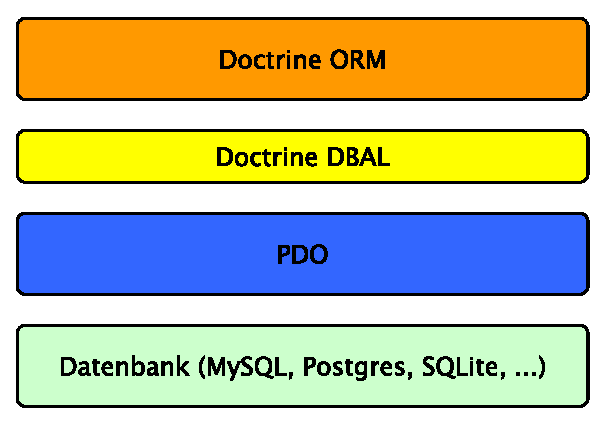
\includegraphics[scale=0.75]{diagrams/DoctrineArchitecture.eps}
    \caption{Schematischer Aufbau von Doctrine}
    \label{fig:doctrineArchitecture}
\end{figure}

\subsection{ORM}
\label{basics:doctrine:subsec:orm}
\begin{shadequote}[l]{Jonathan Wage \cite{web:t3nDoctrine2009}}
	Ein ORM ist eine Abstraktionsschicht zwischen relationaler Datenbank und der eigentlichen Anwendung. Statt per SQL kann man durch das ORM objektorientiert auf die Daten zugreifen.
\end{shadequote}

Das folgende Anwendungsbeispiel zeigt eine typische Situation. Es soll ein neuer Student in die Datenbank der Hochschule eingefügt werden. Im ersten Codelisting wird die Aufgabe auf dem herkömmlichen Weg gelöst. Dabei wird die Anfrage an eine MySQL und PostgreSQL Datenbank gesendet. Die Variable \phpinline{$connection} enthält je eine initialisierte Verbindung zur entsprechenden Datenbank.

\begin{listing}[H]
\begin{phpcode}
<?php

$sql =
    'INSERT INTO students ('first_name', 'last_name', 'enrolment_number')
    VALUES ('Stefano', 'Kowalke', '12345');

// MySQLi
$result = mysqli_query($connection, $sql);

// PostgreSQL
$result = pg_query($connection, $sql);

\end{phpcode}
\caption{Einfügen eines Studenten in die Datenbank ohne ORM}
\label{lst:withoutOrm}
\end{listing}

Im folgenden Listing wird die gleiche Aufgabe mit Doctrine ORM gelöst. Es wird zunächst ein neues Objekt eines Studenten erzeugt und im weiteren Verlauf mit verschiedenen Daten angereichert. Anschließend wird es als zu speicherndes Objekt bei der Datenbank registriert und schlussendlich gespeichert.
\begin{listing}[H]
\begin{phpcode}
<?php

$student = new Student();
$student->setFirstName('Stefano');
$student->setLastName('Kowalke');
$student->setEnrolmentNumber('12345');
$entityManager->persist($student);
$entityManager->flush();
\end{phpcode}
\caption{Einfügen eines Studenten in die Datenbank mit ORM}
\label{lst:orm}
\end{listing}


Der Code in Listing~\ref{lst:orm} gibt keinen Rückschluss auf die darunter liegende Datenbank. Die Daten des Studenten könnten in eine CSV-Datei, einer MySQL oder Postgres Datenbank gespeichert worden sein. Hingegen wurden in Listing~\ref{lst:withoutOrm} zwei verschiedene Methoden genutzt, um die Daten in eine MySQL und Postgres Datenbank zu schreiben. Die Speicherung in eine Textdatei wurde dabei nicht berücksichtigt.

Doctrine ORM ist für die Umwandlung des \phpinline{$student}-Objekt, in eine \gls{sql}-Abfrage zuständig. Die erzeugte Abfrage ist mit der aus Listing~\ref{lst:withoutOrm} vergleichbar. Die Konvertierung der Anfrage in die verschiedenen \gls{glos:sqlDialect} erfolgt durch Doctrine DBAL.

\subsection{DBAL}
\label{basics:doctrine:subsec:dbal}
Doctrine konvertiert das Schema anhand von sehr unterschiedlichen Merkmalen in das \gls{sql} des jeweiligen \gls{dbms}, das zum Verständnis einen etwas tieferen Einstieg in die Eigenheiten der \gls{dbms} erfordern. Da dies den Umfang der Arbeit überschreitet, wurden markante Beispiele gewählt, die den Sachverhalt verdeutlichen.

Datenbankschemata werden in Doctrine von der Klasse \phpinline{Schema} repräsentiert. Im Beispiel wird zunächst eine Instanz dieser Klasse erstellt und anschließend eine neue Tabelle und mehrere Tabellenspalten mit unterschiedlichen Datentypen angelegt. In Zeile 30 wird das Schema in eine \gls{sql}-Abfrage übersetzt. Davor existiert es lediglich als PHP-Objekt bis zum Ende der Laufzeit des Scripts.

Die Variable \phpinline{$myPlatform} enthält die Information über das aktuell benutzte \gls{dbms}.

\begin{listing}[H]
\begin{phpcode}
<?php

$schema = new \Doctrine\DBAL\Schema\Schema();
$beUsers = $schema->createTable('be_users‘);
$beUsers->addColumn('uid', 'integer',
  array('unsigned' => TRUE, 'notnull' => TRUE, 'autoincrement' => TRUE)
);
$beUsers->addColumn('pid', 'integer',
  array('unsigned' => TRUE, 'default' => '0', 'notnull' => TRUE)
);
$beUsers->addColumn('username', 'string',
  array('length' => 50, 'default' => '', 'notnull' => TRUE)
);
$beUsers->addColumn('password', 'string',
  array('length' => 100, 'default' => '', 'notnull' => TRUE)
);
$beUsers->addColumn('admin', 'boolean',
  array('default' => '0', 'notnull' => TRUE)
);
$beUsers->addColumn('history_data', 'text',
  array('length' => 16777215, 'notnull' => FALSE)
);
$beUsers->addColumn('ses_data', 'text',
  array('notnull' => FALSE)
);
$beUsers->setPrimaryKey(array('uid'));
$beUsers->addIndex(array('pid'), 'be_users_pid_idx');
$beUsers->addIndex(array('username'), 'be_users_username');

$queries = $schema->toSql($myPlatform);
\end{phpcode}
\caption{Erstellen eines Schemas mit Doctrine}
\label{lst:createSchema}
\end{listing}

Die beiden Listings \ref{lst:mysqlFromSchema} und \ref{lst:pgsqlFromSchema} zeigen den Inhalt von \phpinline{$queries} – einmal für MySQL und einmal für PostgreSQL.

\begin{listing}[H]
\begin{mysqlcode}
// Der Inhalt von $queries für MySQL
CREATE TABLE `be_users` (
	`uid` int(10) unsigned NOT NULL AUTO_INCREMENT,
	`pid` int(10) unsigned NOT NULL DEFAULT '0',
	`username` varchar(50) COLLATE utf8_unicode_ci NOT NULL DEFAULT '',
	`password` varchar(100) COLLATE utf8_unicode_ci NOT NULL DEFAULT '',
	`admin` tinyint(1) NOT NULL DEFAULT '0',
	`history_data` mediumtext,
	`ses_data` longtext,
	PRIMARY KEY (`uid`),
	KEY `be_users_pid_idx` (`pid`),
	KEY `be_users_username` (`username`)
) ENGINE=InnoDB AUTO_INCREMENT=2 DEFAULT CHARSET=utf8 COLLATE=utf8_unicode_ci;
\end{mysqlcode}
\caption{Das erstellte Schema als MySQL Anfrage}
\label{lst:mysqlFromSchema}
\end{listing}

\begin{listing}[H]
\begin{psqlcode}
// Der Inhalt von $queries für PostgreSQL
CREATE TABLE be_users (
	uid serial NOT NULL,
	pid integer NOT NULL DEFAULT 0,
	username character varying(50) NOT NULL DEFAULT ''::character varying,
	password character varying(100) NOT NULL DEFAULT ''::character varying,
	admin boolean NOT NULL DEFAULT false,
	history_data text,
	ses_data text,
	CONSTRAINT be_users_pkey PRIMARY KEY (uid)
) WITH (
	OIDS=FALSE
);
\end{psqlcode}
\caption{Das erstellte Schema als PostgreSQL}
\label{lst:pgsqlFromSchema}
\end{listing}

Anhand der Beispiele können folgende Konvertierungen abgeleitet werden:

\begin{table}[H]
	\begin{tabularx}{\textwidth}{|X|X|p{0.26\textwidth}|}
		\hline
		Abstraktion                             & MySQL                                  & PostgreSQL\\ \hline
		\phpinline{integer ... auto_increment}  & \sqlinline{INT(10) ... AUTO_INCREMENT} & \sqlinline{serial}\\ \hline
		\phpinline{integer}                     & \sqlinline{INT(10)}                    & \sqlinline{INTEGER} \\ \hline
		\phpinline{string ... length => 50}     & \sqlinline{VARCHAR(50)}                & \sqlinline{CHARACTER VARYING(50)} \\ \hline
		\phpinline{boolean}                     & \sqlinline{TINYINT(1)}                 & \sqlinline{BOOLEAN} \\ \hline
		\phpinline{text ... length => 255}      & \sqlinline{TINYTEXT}                   & \sqlinline{TEXT} \\ \hline
		\phpinline{text}                        & \sqlinline{LONGTEXT}                   & \sqlinline{TEXT}\\ \hline
	\end{tabularx}
	\caption{Typkonvertierung von Doctrine nach MySQL und PostgreSQL}
	\label{tab:typeConvertationDoctrine}
\end{table}

Doctrine wählt die entsprechenden Typen anhand der folgenden Kriterien aus:

\begin{itemize}
	\item Angabe von weiteren Optionen: \phpinline{auto_increment}
	\item Angabe einer Länge: \phpinline{length => 50} bzw. \phpinline{length => 255}
	\item Konvertierung in äquivalente Datentypen: MySQL implementiert keinen \sqlinline{BOOLEAN} Typ, daher wird hier \sqlinline{TINYINT(1)} genutzt
\end{itemize}

Dabei ist zu beachten, dass die Werte in Klammern für String-Typen eine andere Bedeutung haben, als für numerische Datentypen. Wird ein \sqlinline{VARCHAR} mit der Länge 34 definiert, bedeutet dies, dass darin eine Zeichenkette mit maximal 34 Zeichen inklusive Leerzeichen gespeichert werden kann. Würde man auf den Gedanken kommen, in dieser Spalte den kompletten Inhalt des Buches \textit{The Hitchhiker's Guide to the Galaxy} von Douglas Adams speichern zu wollen, würde der Inhalt wie folgt aussehen: ``Far out in the uncharted backwate'' \cite[S. 3]{book:adamsHitchhikers1995}. Der Rest des Textes würde abgeschnitten.

Bei numerischen Datentypen beschreibt der Wert allerdings die Anzeigenbreite - also die Anzahl der angezeigen Ziffern des gespeicherten Wertes. Sollte der in der Spalte gespeicherte Wert kleiner sein als die Länge der Anzeigenbreite, würden die restlichen Stellen nach links mit Leerzeichen aufgefüllt. Wurde die Option \sqlinline{ZEROFILL} gesetzt, würden die restlichen Stellen mit Nullen anstelle von Leerzeichen aufgefüllt. Der Wert beeinflusst in keinster Weise den maximal speicherbaren Wert. In einer als \sqlinline{TINYINT} definierten Spalte können immer 256 Werte gespeichert werden. Unabhängig davon ob sie als \sqlinline{TINYINT(1)} oder \sqlinline{TINYINT(4)} deklariert wurde.

Doctrine spiegelt dieses Verhalten wider, indem die Angabe von \phpinline{length} bei der Deklaration eines Integers dem Wert der Anzeigenbreite entspricht; bei String-Typen den tatsächlichen speicherbaren Wertebereich und bei der Deklaration eines Text-Datentyps als Auswahlkriterium in Bezug auf die unterschiedlichen \sqlinline{TEXT} Datentypen.

\subsection{Unterstützte Datenbank-Plattformen}
\label{basics:doctrine:subsec:supportedPlatforms}
Doctrine unterstützt die folgenden Plattformen und kann um weitere Datenbanken erweitert werden.

\begin{itemize}
		\item DB2
		\item Drizzle
		\item MySQL
		\item Oracle
		\item PostgreSQL
		\item SQLAnywhere
		\item SQLite
		\item SQLAzure
		\item SQL Server
\end{itemize}

\subsection{Konzepte und Architektur von Doctrine}
\label{basics:doctrine:subsec:conceptsAndArchitectureOfDoctrine}
Wie aus Abbildung~\ref{fig:doctrineArchitecture} ersichtlich ist und schon erwähnt wurde, setzt Doctrine DBAL auf \gls{pdo} auf. Im Grunde bildet Doctrine DBAL lediglich eine dünne Schicht auf \gls{pdo}, während \gls{pdo} selbst die Datenbankabstraktion und eine einheitliche API für verschiedene \gls{dbms} zur Verfügung stellt.

\gls{pdo} besteht aus der Klasse \phpinline{PDO}, die eine Verbindung zur Datenbank darstellt, und aus der Klasse \phpinline{PDOStatement}, die zum einen ein (Prepared) Statement als auch das Ergebnis einer Datenbankabfrage repräsentiert. Abbildung~\ref{fig:PDOMainClasses} zeigt die Klassen mit einer Auswahl an Methoden.

\begin{figure}[H]
	\centering
	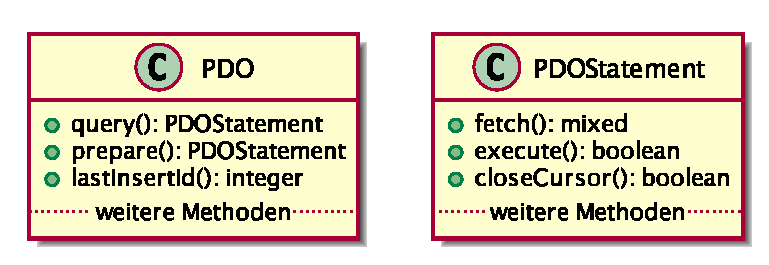
\includegraphics[scale=0.77]{uml/PDOMainClasses.eps}
	\caption{Die beiden PDO-Klassen}
	\label{fig:PDOMainClasses}
\end{figure}

Die äquivalenten Klassen in Doctrine DBAL dazu sind \phpinline{Doctrine\DBAL\Connection} und \phpinline{Doctrine\DBAL\Statement}.

Die Integration der beiden \gls{pdo}-Klassen in Doctrine DBAL erfolgt über das Adapter Entwurfsmuster (siehe Abbildung~\ref{fig:adapterPattern}). Das hat den Vorteil, dass Doctrine DBAL nicht auf \gls{pdo} als Datenbanktreiber festgelegt ist, sondern um weitere Treiber erweitert werden kann. Neue Treiber müssen lediglich das jeweilige Interface implementieren.

\begin{figure}[H]
	\centering
	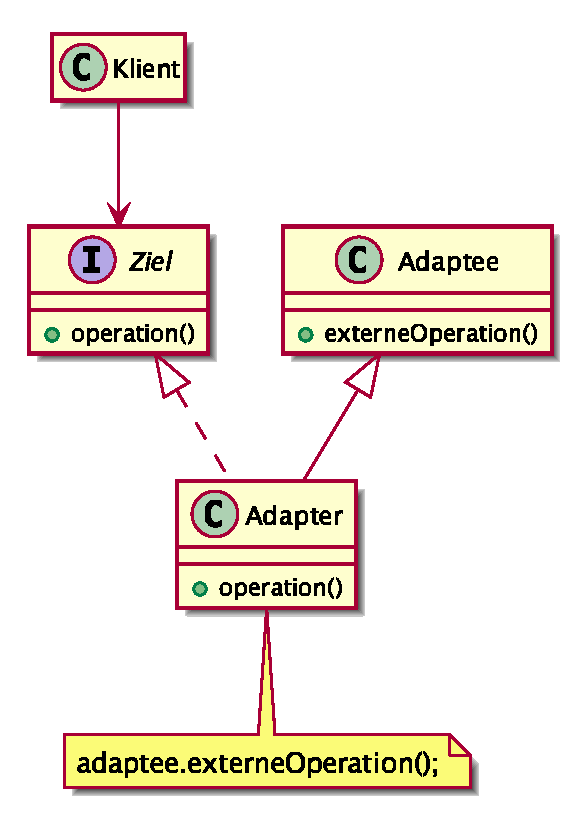
\includegraphics[scale=0.5]{uml/AdapterPattern.eps}
	\caption{Das Adapter Entwurfsmuster in UML-Notation}
	\label{fig:adapterPattern}
\end{figure}

Ein Adapter hat die Aufgabe eine Schnittstelle in eine andere zu konvertieren. Ein Reisestecker oder ein Displayport-zu-VGA-Adapter stellen typische Beispiele aus der realen Welt dar.

In der Softwareentwicklung wird ein Adapter genutzt, wenn eine externe Bibliothek in das eigene Projekt eingebunden werden soll und weder die API des eigenen Projekts noch die der externen Bibliothek verändert werden kann.

Die Akteure innerhalb des Adapter Entwurfsmusters sind:

\begin{itemize}
	\item ein Klient: Stellt die Klasse dar, die die API nutzt. Dazu enthält sie eine interne Variable, die ein Objekt vom Typ des Interfaces erwartet.
	\item ein Ziel: ist ein Interface, welches die zu adaptierenden Methoden definiert. Der Klient wird gegen dieses Interface programmiert.
	\item ein Adapter: Stellt eine konkrete Implementierung des Interfaces dar und ist eine Kindklasse des \gls{glos:adaptee}. Die Methoden des Adapters rufen intern die Methoden der Elternklasse auf, entsprechen nach außen jedoch der vom Klienten erwarteten API
	\item ein \gls{glos:adaptee}: Die zu adaptierende externe Schnittstelle.
\end{itemize}

\newpage

Das UML Diagramm in Abbildung~\ref{fig:adapterPatternConnection} zeigt die Implementation der Connection API, die diesem Muster folgt.

\begin{figure}[H]
	\centering
	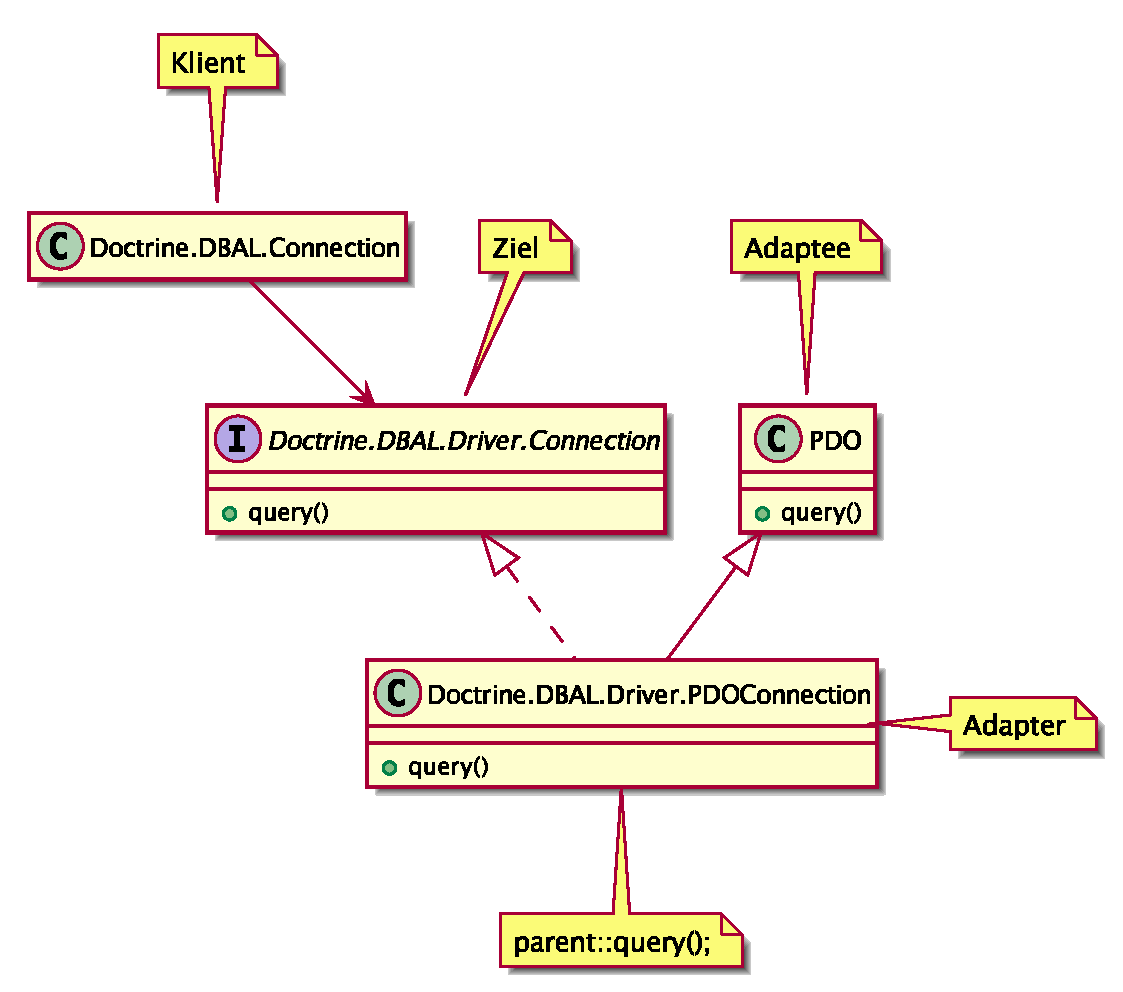
\includegraphics[scale=0.5]{uml/AdapterPatternConnection.eps}
	\caption{Aufbau des Connection-Objekts von Doctrine DBAL}
	\label{fig:adapterPatternConnection}
\end{figure}

Die Klasse \phpinline{Doctrine\DBAL\Connection} stellt die Wrapper-Klasse beziehungsweise den Klienten dar. In der geschützten Variable \phpinline{$_conn} wird ein Objekt erwartet, welches das Interface \phpinline{Doctrine\DBAL\Driver\Connection} erfüllt. Bei \gls{pdo}-basierten Verbindungen ist \phpinline{Doctrine\DBAL\Driver\PDOConnection} ein konkretes Objekt dieses Interfaces. Es erbt außerdem von \phpinline{PDO} und stellt den Adapter dar.

Die Klasse \phpinline{PDOStatement} von \gls{pdo} wird ebenfalls auf diese Art in Doctrine DBAL eingebunden

\begin{figure}[H]
	\centering
	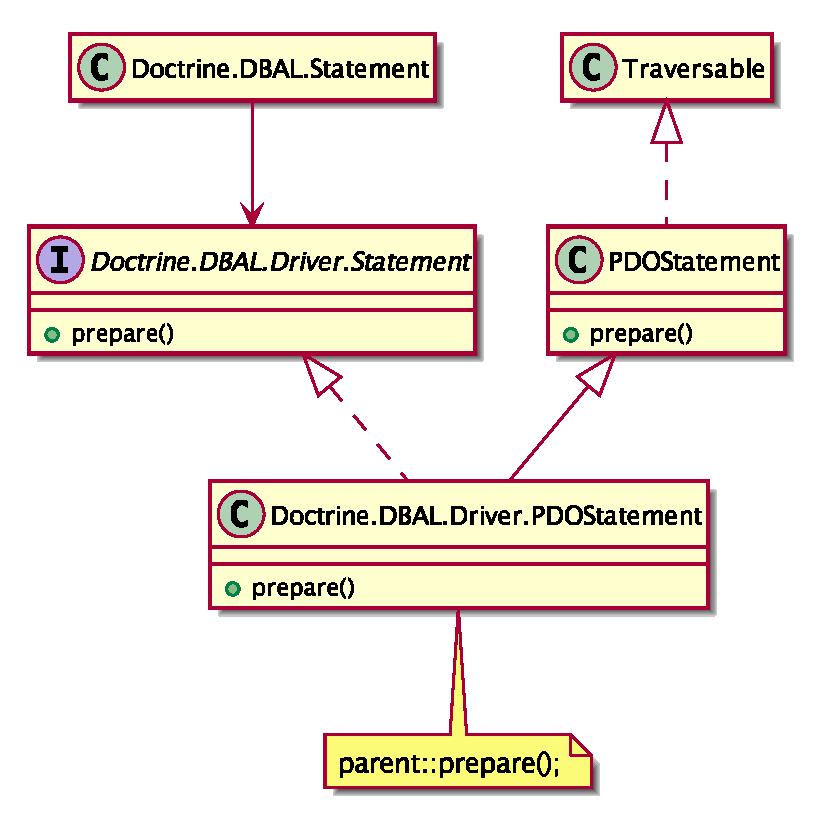
\includegraphics[scale=0.5]{uml/AdapterPatternStatement.eps}
	\caption{Aufbau des Statement-Objekts von Doctrine DBAL}
	\label{fig:adpaterPatternStatement}
\end{figure}

\subsubsection{Verbindung aufbauen}
\label{basics:doctrine:subsubsec:createConnection}
Über \phpinline{Doctrine\DBAL\DriverManager::getConnection()} wird eine Verbindung angefordert. Dies wird in Listing~\ref{lst:DBALConnection} gezeigt.

\begin{listing}[H]
\begin{phpcode}
$config = new \Doctrine\DBAL\Configuration();

$connectionParams = array(
    'dbname' => 'hogwartsDB',
    'user' => 'snape',
    'password' => 'secret',
    'host' => 'localhost',
    'driver' => 'pdo_mysql',
);

$connection = \Doctrine\DBAL\DriverManager::getConnection(
                 $connectionParams,
                 $config
              );
\end{phpcode}
\caption{Aufbau einer Datenbankverbindung mit Doctrine DBAL}
\label{lst:DBALConnection}
\end{listing}

Anhand des angegebenen Wertes in \phpinline{'driver'} wählt Doctrine den entsprechenden Datenbanktreiber aus und erstellt ein \phpinline{PDOConnection}-Objekt, da es sich bei \phpinline{'pdo_mysql'} um eine \gls{pdo}-basierte Verbindung handelt.

Über den zweiten Parameter \phpinline{$config} kann eine Konfiguration an Doctrine DBAL übergeben werden. Außerdem ist es möglich ein \phpinline{Logger}-Objekt zu definieren, welches über dieses Objekt in Doctrine DBAL injiziert wird.

\subsubsection{Einfache Datenbankanfragen}
\label{basics:doctrine:subsubsec:simpleDatabaseQueries}

Im Folgenden wird die Verwendung von Doctrine DBAL an einfachen Beispielen erläutert. Als Grundlage der Abfragen und Ergebnisse dient eine Datenbank mit der folgenden Tabelle. Um die Beispiele einfach zu halten wurde auf eine korrekte Normalisierung der Tabelle, bei der die letzte Spalte in eine eigene Tabelle überführt und per Fremdschlüssel referenziert wird, verzichtet.

\begin{table}[H]
\begin{Verbatim}[samepage=true]
students
+----+------------+-----------+------------+
| id | first_name | last_name |   house    |
+----+------------+-----------+------------+
|  1 | Lucius     | Malfoy    | Slytherin  |
|  3 | Herminone  | Granger   | Gryffindor |
|  4 | Ronald     | Weasley   | Gryffindor |
|  5 | Luna       | Lovegood  | Ravenclaw  |
|  6 | Cedric     | Diggory   | Huffelpuff |
+----+------------+-----------+------------+
\end{Verbatim}
\caption{Auszug aus der Datenbanktabelle}
\label{tab:students}
\end{table}

\newpage

Die als Beispiel dienende Abfrage soll die Nachnamen aller Studierenden in alphabetischer Reihenfolge ausgeben. Die in einer Variablen gespeicherten \gls{sql}-Abfrage wird an die Datenbank gesendet und das Ergebnis über eine Schleife ausgegeben. Zunächst wird der althergebrachte Weg gezeigt. Beide \gls{php}-Extensions stellen dafür \phpinline{*_query} Funktionen zur Verfügung, die eine Kennung der Datenbankverbindung zurückgeben. Im Fall eines Fehlers geben sie \phpinline{FALSE} zurück.

\begin{listing}[H]
\begin{phpcode}
$sql = 'SELECT last_name FROM students ORDER BY last_name';
// For MySQLi:
$result = mysqli_query($connection, $query);
while($row = mysqli_fetch_assoc($result)) {
	echo $row['last_name'] . ' ';
}

// PostgreSQL:
$result = pg_query($query);
while($row = pg_fetch_assoc($result)) {
	echo $row['last_name'] . ' ';
}
\end{phpcode}
\caption{Ausgabe der Studierenden mit MySQL und PostgreSQL}
\label{lst:externalFetchAssocMethods}
\end{listing}

In Doctrine DBAL enthält \phpinline{Doctrine\DBAL\Connection} die Verbindung zur Datenbank. Um eine Anfrage an die Datenbank zu senden, bietet die Klasse die Methode \phpinline{query()} an. Die Methode gibt ein Objekt vom Typ \phpinline{Doctrine\DBAL\Statement} zurück, dass das \phpinline{IteratorAggregate} Interface implementiert. Dadurch kann über das Objekt mittels einer \phpinline{foreach}-Schleife iteriert werden.

\begin{listing}[H]
\begin{phpcode}
$sql = 'SELECT last_name FROM students ORDER BY last_name';

$statement = $connection->query($sql);

foreach($statement as $row) {
  echo $row['last_name'] . ' ';
}
\end{phpcode}
\caption{Einfache Datenbankabfrage mit Doctrine DBAL}
\label{lst:dbalSimpleQuery}
\end{listing}

Die Ausgabe aller Beispiele lautet:
\begin{Verbatim}
Diggory Granger Lovegood Malfoy Weasley
\end{Verbatim}

\newpage

\subsubsection{Funktionen auf der Ergebnismenge}
\label{basics:doctrine:subsubsec:resultSet}
Um das Ergebnis der Abfrage sinnvoll nutzen zu können, gibt es verschiedene Formate (engl. fetch styles) in denen das Ergebnis ausgegeben werden kann. In dem Listing~\ref{lst:dbalSimpleQuery} wird die Standardeinstellung \phpinline{PDO:FETCH_BOTH} genutzt. Dabei kann auf die Werte sowohl über einen Index als auch über den Spaltenbezeichner zugegriffen werden. Die interne Struktur sieht wie folgt aus:

%\begin{listing}[H]
%\begin{phpcode}
%foreach($statement as $row) {
  %print_r($row);
%}
%\end{phpcode}
%\caption{}
%\label{lst:internalStructureOfFetchBoth}
%\end{listing}

\begin{Verbatim}
Array
(
    [last_name] => Diggory
    [0] => Diggory
)
Array
(
    [last_name] => Granger
    [0] => Granger
)
Array
(
    [last_name] => Lovegood
    [0] => Lovegood
)
...
\end{Verbatim}

Die Formatierung der Ergebnismenge wird über Konstanten gesteuert, die von \gls{pdo} definiert und an die Methode \phpinline{query()} als optionales Argument übergeben werden können. Eine andere Konstante ist \phpinline{PDO:FETCH_NUM}, die das Ergebnis in ein Index-basiertes Array formatiert.

\begin{listing}[H]
\begin{phpcode}
$statement = $connection->query($sql, PDO::FETCH_NUM);

foreach($statement as $row) {
  echo $row[0];
}
\end{phpcode}
\caption{Steuerung der Formatierung der Ergebnismenge}
\label{lst:fetchNum}
\end{listing}

In \gls{pdo} existiert für jede Fetch-Methode aus der traditionellen Datenbankprogrammierung ein Äquivalent in Form einer Konstante:

\begin{itemize}
	\item \phpinline{PDO::FETCH_ASSOC} = \phpinline{*_fetch_assoc()}\footnote{Der Stern (*) dient als Platzhalter und kann wahlweise durch mysql, mysqli oder pg ersetzt werden.}
	\item \phpinline{PDO::FETCH_NUM} = \phpinline{*_fetch_array()}
	\item \phpinline{PDO::FETCH_ROW} = \phpinline{*_fetch_row()}
\end{itemize}

Über das \phpinline{Doctrine\DBAL\Statement}\footnote{Leider ist der Begriff dieser Klasse etwas unglücklich gewählt oder es ist ein Designfehler von \gls{pdo}, denn ein Objekt dieser Klasse repräsentiert zum einen ein (Prepared) Statement und, nachdem die Anfrage ausgeführt wurde, die Ergebnisrelation. Die Methoden der Klasse agieren somit einmal auf dem Statement und einmal auf dem Ergebnis. Dies widerspricht dem Konzept in der Objekt-orientierten Programmierung, dass eine Klasse nur eine Verantwortlichkeit (engl. Single Responsibility Principle) haben darf. (vgl. \cite[S. 181]{book:martinCleanCode2008})} werden weitere Möglichkeiten wie die Methoden \phpinline{Doctrine\DBAL\Statement::fetch()} und \phpinline{Doctrine\DBAL\Statement::fetchAll()} angeboten, um das Ergebnis zu erhalten.

\begin{listing}[H]
\begin{phpcode}
$statement = $connection->query($sql);

while($row = $statement->fetch(PDO::FETCH_ASSOC)) {
  echo $row['last_name'];
}
\end{phpcode}
\caption{Übergabe der Konstante an die fetch()-Methode}
\label{lst:fetctWithWhileLoop}
\end{listing}

\subsubsection{Prepared Statements}
\label{basics:doctrine:subsubsec:preparedStatements}
Prepared Statements wurden bereits von der Datenbankerweiterung MySQLi eingeführt und sind keine Neuheit in der \gls{php} Welt. Während MySQLi nur einen Typ der Prepared Statements unterstützt, stellt \gls{pdo} eine weitere Variante zur Verfügung. Mit Doctrine DBAL können beide Ansätze genutzt werden.

Prepared Statements stellen normalen \gls{sql}-Code dar, bei dem die variablen Teile durch Platzhalter ersetzt wurden. Sie können als eine Vorlage für \gls{sql}-Abfragen verstanden werden, die mit verschiedenen Werten immer wieder ausgeführt werden sollen.

Ein Prepared Statement wird zunächst an die Datenbank gesendet, wo der \gls{sql}-Parser die Struktur des Templates einmalig analysieren und vorkompiliert im Cache speichern kann. In einer zweiten Anfrage werden der Datenbank die Werte übermittelt, die bei jedem erneuten Aufruf vom Parser anstelle der Platzhalter eingesetzt werden. Dies macht zum einen die Ausführung der Anfrage schneller (vgl. \cite[S. 75]{book:popel2007pdo}) und erhöht zudem die Sicherheit, da es \gls{sql}-Injections nahezu unmöglich macht. Mehr zu \gls{sql}-Injections in Kapitel~\ref{basics:doctrine:subsubsec:sqlInjections}.

Zur Demonstration soll je ein Codebeispiel dienen. Dabei werden neue Studierende in die oben gezeigte Datenbanktabelle eingefügt. Der sprechende Hut\footnote{\url{http://de.harry-potter.wikia.com/wiki/Sprechender_Hut}} hat bereits über die Häuser der Neuzugänge entschieden.

Die Daten der Studierenden liegen in einem assoziativen Array vor und können somit über eine \phpinline{foreach}-Schleife durchmustert werden. Pro Schleifendurchlauf wird ein Studierender der Datenbank hinzugefügt. Die Werte werden durch\\
\phpinline{Doctrine\DBAL\Connection::quote()} maskiert, um \gls{sql}-Injections zu unterbinden.

In Listing~\ref{lst:lst:insertWithoutPreparedStatement} wird bei jedem Durchlauf eine neue Abfrage mit den aktuellen Daten erzeugt und an die Datenbank geschickt. Für diese wiederkehrende Aufgabe bietet sich die Benutzung von Prepared Statements an, da pro Iteration lediglich die Werte angepasst werden müssen.

\begin{listing}[H]
\begin{phpcode}
$students = array (
	array (
		'last_name' => 'Ellesmere',
		'first_name' => 'Corin',
		'house' => 1
	),
	array (
		'last_name' => 'Tugwood',
		'first_name' => 'Havelock',
		'house' => 4
	),
	array (
		'last_name' => 'Fenetre',
		'first_name' => 'Valentine',
		'house' => 3
	)
)

foreach ($students as $student) {
	$sql = 'INSERT INTO students (last_name, first_name, house)
	  VALUES (' . $connection->quote($student['last_name']) .
	    ',' . $connection->quote($student['first_name']) .
	    ',' . $connection->quote($student['house']) . ')');

	$connection->query($sql);
}
\end{phpcode}
\caption{INSERT Abfrage ohne Prepared Statements}
\label{lst:insertWithoutPreparedStatement}
\end{listing}

Das folgende Listing~\ref{lst:insertWithPreparedStatementPosParams} verwendet anstelle der eigentlichen Daten Fragezeichen als Platzhalter, die als \textit{Positional Placeholders} bezeichnet werden. Die Daten werden der Methode \phpinline{Doctrine\DBAL\Statement::execute()} in einem Array übergeben. Dabei ist die Reihenfolge wichtig, da ansonsten die Daten in die falschen Spalten der Tabelle geschrieben werden. Bei der Benutzung von Prepared Statements kann auf die Maskierung durch \phpinline{Doctrine\DBAL\Connection::quote()} verzichtet werden, da dies die Datenbank übernimmt.
\begin{listing}[H]
\begin{phpcode}
$statement = $connection->prepare(
  'INSERT INTO students (last_name, first_name, house)
    VALUES (?, ?, ?)');

foreach ($students as $student) {
	$statement->execute(
	  array(
	    $student['last_name'],
	    $student['first_name'],
	    $student['house']);
	);
}
\end{phpcode}
\caption{Prepared Statements mit Positional Parameter}
\label{lst:insertWithPreparedStatementPosParams}
\end{listing}

\newpage

\gls{pdo} bietet - im Gegensatz zu MySQLi - mit den \textit{Named Parametern} noch eine weitere Möglichkeit für Platzhalter an. Anstelle von Fragezeichen werden Bezeichner mit einem vorangestellten Doppelpunkt verwendet. Der Vorteil dieser Variante ist, dass die Reihenfolge bei der Übergabe der Daten an \phpinline{Doctrine\DBAL\Statement::execute()} keine Rolle mehr spielt. Das folgende Listing zeigt den gleichen Code aus Listing~\ref{lst:insertWithPreparedStatementPosParams} jedoch diesmal mit \textit{Named Parametern}. Die Daten werden dieses Mal als Key-/Value-Paar übergeben, bei dem der \textit{Key} den benannten Platzhalter darstellt und der \textit{Value} die einzufügenden Werte.

\begin{listing}[H]
\begin{phpcode}
$statement = $connection->prepare(
  'INSERT INTO students (last_name, first_name, house)
    VALUES (:lastname, :firstname, :house)');

foreach ($students as $student) {
	$statement->execute(
	  array(
	    ':firstname' => $student['first_name'],
	    ':lastname'  => $student['last_name'],
	    ':house'     => $student['house']);
	);
}
\end{phpcode}
\caption{Prepared Statements mit Named Parameter}
\label{lst:insertWithPreparedStatementNamedParams}
\end{listing}

\subsubsection{Binding}
\label{basics:doctrine:subsubsec:binding}
Die Zuordnung einer Variablen zu einem Platzhalter wird \textit{Binding} genannt - gebundene Variablen werden demzufolge als \textit{Bounded Variables} bezeichnet.

Neben der gezeigten Bindung über \phpinline{PDOStatement::execute()} bietet \gls{pdo} spezialisierte Methoden an, was folgende Ursachen hat:

\begin{enumerate}
	\item Bei der gezeigten Bindung werden die Variablen stets als String behandelt. Es ist nicht möglich dem \gls{dbms} mitzuteilen, dass der übergebene Wert einem anderen Datentyp entspricht.
	\item Die Variablen werden bei dieser Methode stets als In-Parameter übergeben. Auf den Wert der Variablen kann innerhalb der Funktion nur lesend zugegriffen werden. Man nennt diese Übergabe auch \textit{by Value}. Es gibt jedoch Szenarien in denen der Wert der Variable innerhalb der Funktion geändert werden soll. Dann müssen die Parameter als Referenz (\textit{by Reference}) übergeben werden und agieren als In/Out-Parameter. Einige \gls{dbms} unterstützen dieses Vorgehen und speichern das Ergebnis der Abfrage wieder in der übergebenen Variable.
\end{enumerate}

Das Äquivalent zum obigen Beispiel ist \phpinline{Doctrine\DBAL\Statement::bindValue()}, bei der die Variable als In-Parameter übergeben wird. Für jeden zu bindenden Platzhalter muß die Methode aufgerufen werden, die dessen Bezeichner, den zu bindenden Wert und die optionale Angabe des Datentyps erwartet. Der Datentyp wird der Datenbank über \gls{pdo}-Konstanten mitgeteilt. \phpinline{PDO::PARAM_STR} ist der Standardwert des zweiten Parameters.

\begin{listing}[H]
\begin{phpcode}
$statement = $connection->prepare(
  'INSERT INTO students (last_name, first_name, house)
    VALUES (:lastname, :firstname, :house)');

foreach ($students as $student) {
    $statement->bindValue(':lastname', $student['first_name']);
    $statement->bindValue(':firstname', $student['last_name']);
    $statement->bindValue(':house', $student['house'], PDO::PARAM_INT);

	$statement->execute();
}
\end{phpcode}
\caption{}
\label{lst:insertBindValue}
\end{listing}

Die Methode \phpinline{Doctrine\DBAL\Statement::bindParam()} unterscheidet sich dazu grundlegend. Der in der Variable gespeicherte Wert wird erst dann aus dem Speicher ausgelesen, wenn \phpinline{Doctrine\DBAL\Statement::execute()} ausgeführt wird. Im Vergleich dazu wird der Wert schon bei dem Aufruf von \phpinline{Doctrine\DBAL\Statement::bindValue()} vom \gls{sql}-Parser ausgelesen und in das Prepared Statement eingesetzt. Aus diesem Grund muß \phpinline{Doctrine\DBAL\Statement::bindValue()} innerhalb der Schleife aufgerufen werden.

\begin{listing}[H]
\begin{phpcode}
$statement = $connection->prepare(
  'INSERT INTO students (last_name, first_name, house)
    VALUES (:lastname, :firstname, :house)');

$statement->bindParam(':lastname', $student['first_name']);
$statement->bindParam(':firstname', $student['last_name']);
$statement->bindParam(':house', $student['house'], PDO::PARAM_INT);

foreach ($students as $student) {
	$statement->execute();
}
\end{phpcode}
\label{lst:insertBindParam}
\end{listing}

\newpage

\subsubsection{SQL-Injections}
\label{basics:doctrine:subsubsec:sqlInjections}
\begin{figure}[H]
    \centering
    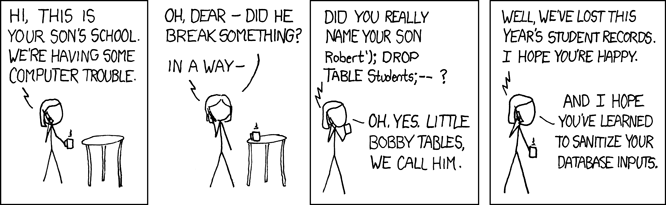
\includegraphics[scale=0.5]{exploits_of_a_mom.png}
    \caption{xkcd: Exploits of a mom\footnotemark}
    \label{fig:littleBobbyTables}
\end{figure}
\footnotetext{\url{http://xkcd.com/327/}}
Bei \gls{sql}-Injections kann über das Frontend einer Anwendung eine Zeichenkette in eine \gls{sql}-Abfrage injiziert werden, die die Fähigkeit besitzt den betroffenen \gls{sql}-Code derart zu verändern, dass er

\begin{itemize}
	\item Informationen wie den Administrator der Webanwendung zurückliefert
	\item Daten in der Datenbank manipuliert
	\item oder die Datenbank ganz- oder teilweise löscht
\end{itemize}

Für ein kurzes Beispiel einer \gls{sql}-Injection soll ein Formular dienen, in dem nach den Nachnamen der Studierenden aus Hogwarts gesucht werden kann. Der gesuchte Datensatz wird ausgegeben wenn er gefunden wird, ansonsten erscheint eine entsprechende Meldung, dass nichts gefunden wurde. Der in das Eingabefeld eingegebene Wert wird von \gls{php} automatisch in der Variablen \phpinline{$_REQUEST} gespeichert und kann in der Anwendung ausgelesen werden. \phpinline{'SELECT * FROM students WHERE last_name = Diggory'} stellt eine mögliche, zu erwartende \gls{sql}-Abfrage dar.

\begin{listing}[H]
\begin{phpcode}
$sql = "SELECT * FROM students
  WHERE last_name = '" . $_REQUEST['lastName'] . "'";

$statement = $connection->query($sql);

foreach($statement as $student) {
  echo 'Lastname: ' . $student['last_name'] . "\n";
  echo 'Firstname: ' . $student['first_name'] . "\n";
  echo 'Haus: ' . $student['house'] . "\n";
}
\end{phpcode}
\caption{}
\label{lst:sqlInjections}
\end{listing}

Dieser Code beinhaltet zwei Fehler:

\begin{enumerate}
	\item Es wird nicht überprüft, ob \phpinline{$_REQUEST['lastName']} leer ist oder etwas ganz anders enthält als erwartet, wie zum Beispiel ein Objekt oder Array.
	\item die Benutzereingabe wird nicht maskiert
\end{enumerate}

Im Falle einer leeren Variable, sähe die Abfrage so aus:\\ \phpinline{'SELECT * FROM students WHERE last_name = '}.

Im besten Fall gibt sie eine leere Ergebnismenge zurück, im schlechtesten einen Fehler. Dieses Problem ist leicht zu lösen, indem zum einen auf die Existenz der Variablen geprüft wird und zum anderen, ob sie einen Wert enthält. Zusätzlich sollte noch auf den Datentyp des enthaltenen Wertes geprüft werden. Erst dann wird die Anfrage abgesetzt.

Da die Eingabe nicht maskiert wird, interpretiert der \gls{sql}-Parser einige Zeichen als Steuerzeichen der \gls{sql}-Syntax. Beispiele solcher Zeichen sind das Semikolon (\pdf{;}), der Apostroph (\pdf{'}), der Backslash (\pdf{\textbackslash}) oder zwei Minuszeichen (\pdf{--}).

Selbst ein Websitebesucher ohne kriminelle Absichten könnte mit der Suche nach einem Studenten mit dem Namen \textit{O'Hara} die \gls{sql}-Injection auslösen. Die in diesem Fall an die Datenbank gesendete \gls{sql}-Abfrage \phpinline{'SELECT * FROM students WHERE last_name = 'O'Hara';} würde wohl einen Fehler auslösen, da der Parser die Anfrage nach dem \textit{O} anhand des Apostroph als beendet interpretiert und \phpinline{Hara} kein gültiges Sprachkonstrukt von \gls{sql} darstellt.

Ein Angreifer könnte hingegen die Eingabe in das Formular nach \mysqlinline{' or '1'='1} verändern. Damit würde sich diese Abfrage\\ \mysqlinline{'SELECT * FROM students WHERE last_name = '' or '1'='1';} ergeben.

Wird die Maskierung mit einer entsprechenden Prüfung von Benutzereingaben kombiniert, verhindert das die Gefahr von \gls{sql}-Injections – eine richtige Anwendung vorausgesetzt.

Die an \phpinline{Doctrine\DBAL\Connection::query()} übergebenen \gls{sql}-Abfragen müssen durch \phpinline{Doctrine\DBAL\Connection::quote()} maskiert werden. Traditionell wird dafür die \gls{php}-Funktion \phpinline{addslashes()} oder die jeweiligen Maskierungsmethoden der \gls{dbms} verwendet. Werden Prepared Statements genutzt, müssen die Benutzereingaben trotzdem überprüft, jedoch nicht mehr maskiert werden. Dies übernimmt der \gls{sql}-Parser, der lediglich die Werte in das vorkompilierte Prepared Statement einsetzt. Wird dem Prepared Statement noch der Typ des Wertes mitgeteilt, kann das \gls{dbms} eine Typprüfung vornehmen und ggf. einen Fehler zurückgeben.

\subsubsection{Limitierungen}
\label{basics:doctrine:subsubsec:limitsOfAbstraction}
Bei einer Abstraktion wird stets etwas Spezifisches, durch das Weglassen von Details, in etwas Allgemeines überführt. Doctrine DBAL geht den umgekehrten Weg – es werden allgemeine \gls{sql}-Abfragen in den \gls{glos:sqlDialect} des Herstellers übersetzt.

Aus diesem Grund vermag es \gls{pdo}, nicht eine \gls{sql}-Abfrage, die in dem \gls{glos:sqlDialect} eines Herstellers formuliert wurde, in den eines anderen zu übersetzen.

Das folgende Beispiel zeigt die von MySQL unterstützte Form eines \sqlinline{INSERT}-Statements. Dies stellt eine Abweichung vom \gls{sql}-Standard dar (vgl. \cite[S. 388]{website:SQLStandard1992}) und ist somit nicht portabel.

\begin{listing}[H]
\begin{mysqlcode}
INSERT INTO students SET last_name='Kowalke', first_name='Stefano';
\end{mysqlcode}
\caption{}
\label{lst:notPortableSQL}
\end{listing}

Stattdessen muss die Anfrage so nah wie möglich am Standard gestellt werden, um als portabel zu gelten.

\begin{listing}[H]
\begin{mysqlcode}
INSERT INTO students (last_name, first_name) VALUES('Kowalke', 'Stefano');
\end{mysqlcode}
\caption{}
\label{lst:portableSQL}
\end{listing}
